% BDEC system actors & flow — User / TA / Verifier / blockchain ledger.
% Grounded in ProSec2024 §4: IssueCre, CreGen, ShowCre, ShowVer; ledgers rt_cred/rt_TA/RL.
% Shows which steps the zkVM proof of this thesis realises.
% Compile: pdflatex bdec_actors.tex
\documentclass[border=4pt]{standalone}
\usepackage{tikz}
\usepackage{newtxtext,newtxmath}
\usetikzlibrary{positioning,arrows.meta,calc}
\begin{document}
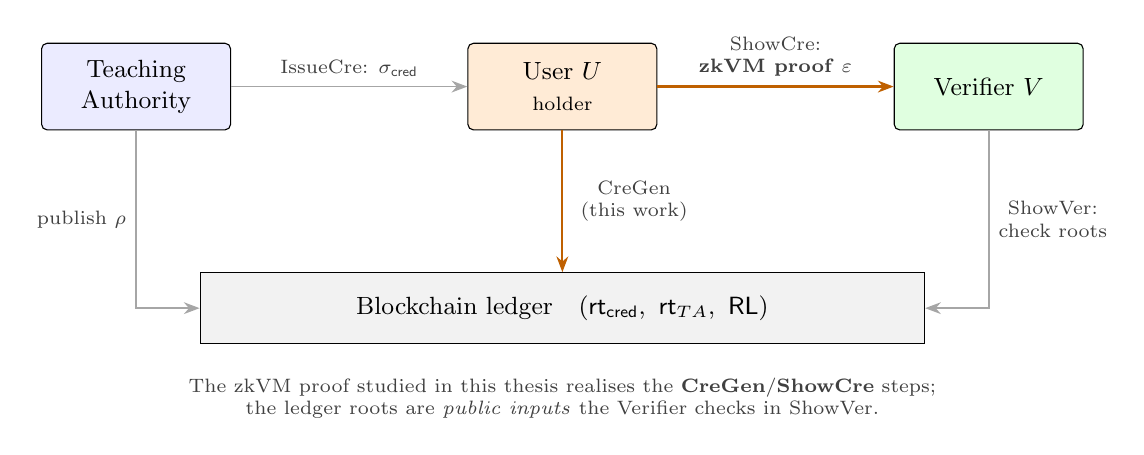
\begin{tikzpicture}[
  font=\small,>={Stealth[length=2mm]},
  actor/.style={draw,rounded corners=2pt,minimum width=24mm,minimum height=11mm,align=center},
  ta/.style={actor,fill=blue!8},
  usr/.style={actor,fill=orange!16},
  ver/.style={actor,fill=green!12},
  ledg/.style={draw,fill=gray!10,minimum width=92mm,minimum height=9mm,align=center},
  slbl/.style={font=\scriptsize,align=center,gray!50!black},
  flow/.style={->,semithick,gray!70},
  zk/.style={->,thick,orange!75!black},
]
\node[usr] (usr) {User $U$\\\scriptsize holder};
\node[ta,left=30mm of usr] (ta) {Teaching\\Authority};
\node[ver,right=30mm of usr] (ver) {Verifier $V$};
\node[ledg,below=18mm of usr] (chain) {Blockchain ledger\quad $(\mathsf{rt}_{\mathsf{cred}},\ \mathsf{rt}_{TA},\ \mathsf{RL})$};

\draw[flow] (ta) -- node[slbl,above]{IssueCre: $\sigma_{\mathsf{cred}}$} (usr);
\draw[zk]   (usr) -- node[slbl,above]{ShowCre:\\\textbf{zkVM proof} $\varepsilon$} (ver);
\draw[flow] (ta.south) |- (chain.west) node[slbl,pos=0.25,left]{publish $\rho$};
\draw[zk]   (usr.south) -- (chain.north) node[slbl,midway,right,xshift=1mm]{CreGen\\(this work)};
\draw[flow] (ver.south) |- (chain.east) node[slbl,pos=0.25,right]{ShowVer:\\check roots};

\node[slbl,below=3mm of chain,align=center]
  {The zkVM proof studied in this thesis realises the \textbf{CreGen}/\textbf{ShowCre} steps;\\
   the ledger roots are \emph{public inputs} the Verifier checks in ShowVer.};
\end{tikzpicture}
\end{document}
